\section{Results \& Evaluations}
In this chapter, we perform evaluation on our model and the other algorithms, the repository of our model is provided in github \footnote{\url{https://github.com/cwleung/LKJTM}}.
\subsection{Experiment Testing}
The experiment will be conducted with a number of existing proposed topic models as mentioned related work section above. We conduct the experiment with those baseline algorithms and evaluate them in terms of accuracy and running time. Some of the source code of competitive were provided by their authors in Github\footnote{For instance, Correlated Topic Model(CTM), \href{https://github.com/blei-lab/ctm-c}{https://github.com/blei-lab/ctm-c}}. The outcome result will be extensively studied and conclude the insight behind the algorithms and methodologies. Detail to be stated in section \ref{AD}. Our probabilistic part of model implemented using Pyro\cite{bingham_pyro_2019}, while the model optimization and transformer implementations are based on PyTorch\cite{paszke_automatic_2017}.
\subsection{Dataset}To evaluate the performance of the model, we selected \textit{20Newsgroups} and \textit{Reuters-21578} data sets in our evaluation stage. 20Newsgroups consist of 18,846 news group documents \footnote{\url{http://qwone.com/~jason/20Newsgroups/}} and the Reuters-21578 includes 10,788 documents in total. Both of the dataset will be preprocessed to remove stop-words and stemming before the evaluation. Both data set were separated into training/testing set for training and evaluation process. 
% 20newsgroups
\textit{20Newsgroups} data set contains around 20,000 newsgroups documents, which divided into 20 different groups. In the preprocessing stage, we remove the document with only one word. We filter the stop-words, remove the word with special characters. The frequency of words are limited to between 2\%-70\%. After the preprocessing, the data set was split into 11314, 7532 documents with 5453 vocabularies. 
% reuter 21578
\textit{Reuter-21578} data set is a collection of documents from Reuters newswire in 1987. After performing the preprocessing, the processed data set consist of 7769, 3019 documents for train/test documents with 1623 vocabularies.
\subsection{Data Preprocessing}
We perform data preprocessing, tokenization, stopword removal, lemmatization, and set the 
\subsection{Models}
We compare the model performance with a numbers of rivals. We take Latent Dirichlet Allocation (LDA)\cite{blei_latent_2003} as the baseline model. Other models include Transformer\cite{vaswani_attention_nodate}\footnote{Not a topic model, but we think it is worth to make comparison still.},  ProdLDA\cite{srivastava_autoencoding_2017} and Embedded Topic Model(ETM)\cite{dieng_topic_2019}.
% LDA
LDA model with mean-field inference \footnote{Adopted from \textmd{scikit-learn} library}
% ProdLDA
ProdLDA, a topic model learning using amortized inference 
% ETM
ETM model, a topic model built on top of ProdLDA model, uses dot-product of word embedding and topic embedding to represent the topic-word distribution $ \beta $.
\subsection{Algorithmic Settings}
% optimization algorithm
To perform posterior inference, we employed Stochastic Variational Inference (SVI) \cite{hoffman_stochastic_2013} for the optimization problem. We set the minibatch size to 1024 documents.
% Other model
For LDA, we applied the model provided from sklearn package (version 0.24.0) \footnote{Sklearn website \url{https://scikit-learn.org/stable/index.html}}. For ETM, we run the experiment with the parameter suggested \cite{dieng_topic_2019}. For ProdLDA, we perform optimization with inference network architecture as described in the paper \cite{srivastava_autoencoding_2017}. 
% epochs
To train the models, every model run on 200 epochs to give the best performance. 
% learning rate
To perform optimization, we use Adam for the gradient ascent algorithm, and we set the learning rate to 2e-3.
% l2-regularization factor
we use $ l2 $-regularization to the 1e-5,
% inference network [size, activation function, dropout, batch-norm]
We applied the settings from \cite{srivastava_autoencoding_2017} to perform amortized inference. The inference architecture included 100 dimension of hidden layers. 
% embedding dimension 512
The dimension for embedding $ \rho $ are set to 128.
% Transformer settings
For the Transformer model settings, we define the sequence length to 20, number of head to 8, and 6 layer stacks of transformer encoder and 128 hidden dimension.
\subsection{Quantitative Result}
In this section, we evaluate the model with the following metric adopted from \cite{dieng_dynamic_2019}: Perplexity, Topic Coherence (TC), Topic Diversity (TD). %and Topic Quality (TQ).\begin{center}
\begin{table}[h]
\centering
\begin{tabular}{lllllll}
\hline
\#Topic     & \multicolumn{3}{c}{k=20} & \multicolumn{3}{c}{k=50} \\
Metrics     & PPL      & TC      & TD  & PPL      & TC      & TD  \\
\hline
LDA         & 2425.9   & 0.183   &  0.754   & \textbf{2521.7}   & 0.149   & 0.742    \\
ProdLDA     & 5652.0   & 0.107   &   0.906  & 5654.1   & 0.074   &     \\
ETM         & \textbf{2709.7}   & 0.153   &  0.486   & 2729.2   & 0.132   & 0.265    \\
Our model   & 3444.1   & \textbf{0.206}   &     & 3705.0   & \textbf{0.199}   &    \\
\hline
\end{tabular}
\captionof{table}{Result for 20Newsgroups dataset\label{tbl:result1}}
\end{table}
\begin{table}[h]
\centering
\begin{tabular}{lllllll}
\hline
\#Topic     & \multicolumn{3}{c}{k=20} & \multicolumn{3}{c}{k=50} \\
Metrics     & PPL     & TC     & TD    & PPL     & TC     & TD    \\ \hline
LDA         & 464.5   & 0.204  & 0.692 & \textbf{510.1}   & 0.155  &  0.580     \\
ProdLDA     & 1599.3  & -0.38  & \textbf{0.872} & 1568.3  & -0.411 & \textbf{0.686} \\
ETM         & \textbf{375.3}   & 0.207  & 0.382 & 629.9   & 0.127  & 0.113 \\
Our model   & 826.3   & \textbf{0.250}  & 0.69  & 805.5   & \textbf{0.253}  & 0.508 \\ \hline
\end{tabular}
\captionof{table}{Result for Reuters-21578 dataset\label{tbl:result2}}
\end{table}
\paragraph{20Newsgroups}On the result from table \ref{tbl:result1}, display that our model has outperform the other model by TC score. On perplexity score, ETM obtain the best score when $ k=20 $ and LDA when $ k=50 $. Since Transformer is not a topic model actually, it got a negative score on TC, which refers it cannot retrieve any useful topic from documents.
\paragraph{Reuters-21578}
% Reuter-21578
On the dataset Reuter-21578, the LDA perform the best in perplexity and ETM when $ k=50 $. And our model still perform the best on topic coherence on both number of topic. 
%
Apparently our model outcome a relatively high topic coherence score but a high perplexity. To investigate the problem, we analyze the metric performance per training epoch.

\subsection{Training}
From figure \ref{fig:loss_20ng_20t}, \ref{fig:loss_20ng_50t}, display the training process of the training loss and log probability by 200 epochs. From \ref{fig:eval_20ng_20t}, \ref{fig:eval_20ng_50t}, we observe that the TD score and TC score increase monotonically, however, the perplexity increases throughout the epochs. 
\subsection{Qualitative Result}The proposed model will be evaluated with a number of specifically selected topic and examined with their performance separately. The result will be exhaustively compared with other existing models.\\
From table \ref{tbl:t3}, we have selected some topic words each model generated from 20Newsgroups when $ k=20 $. The topics represent space, operating system, religion, encryption and guns respectively. Our model has shown capability on capturing key words from each topic, such as on topic "space": \textit{nasa}, \textit{space}, \textit{jpl}, \textit{moon}, \textit{earth}, \textit{station}, \textit{flight} are the outputs.
\begin{table}[ht]
\centering
%\scriptsize
\begin{tabular}{llll}
\hline
Our Model  \\ \hline
\textbf{nasa }gov \textbf{space jpl moon earth station flight }research digex\\
\textbf{windows window }problem \textbf{dos }running \textbf{file mouse }mit de ms\\
\textbf{god jesus christian }people faith bible time church good things\\
\textbf{key }chip \textbf{encryption }clipper \textbf{security }\textbf{privacy }government \textbf{keys }public escrow\\
\textbf{gun }people control government \textbf{guns weapons }american make clinton state \\ \hline
\hline
ProdLDA  \\ \hline
\textbf{nasa} \textbf{space} gov people \textbf{station} \textbf{time} \textbf{orbit} dc program shuttle \\
\textbf{scsi} \textbf{drive} \textbf{controller} max \textbf{drives} \textbf{ide} senior \textbf{tape} time people \\
\textbf{god jesus atheists christian bible religion atheism christians} word truth \\
\textbf{key crypto} session nt chips chip \textbf{serial} dos \textbf{keys} \textbf{encrypted} \\
\textbf{gun }people god religion writes life morality ohio argument question \\ \hline
\hline
LDA  \\ \hline
\textbf{space, nasa}, gov, access, \textbf{launch, earth}, digex, \textbf{moon, orbit}\\
\textbf{file, window, program, ftp}, \textbf{files}, \textbf{server}, \textbf{image, graphics, windows}\\
\textbf{god}, people, \textbf{jesus}, \textbf{christian}, \textbf{bible}, writes, life, \textbf{christians}, time\\
\textbf{key}, \textbf{encryption}, chip, clipper, \textbf{keys}, \textbf{security}, \textbf{government}, \textbf{privacy}\\
\textbf{gun, guns, law, police}, people, \textbf{weapons, crime, fbi}, control
\\ \hline
\hline
ETM  \\ \hline
\textbf{space, nasa}, gov, mr, president, health, research, year, center\\
\textbf{windows, file, window, program, files, server}, \textbf{version}, dos, \textbf{image}\\
\textbf{god}, people, \textbf{jesus}, \textbf{christian}, \textbf{israel}, \textbf{bible}, \textbf{jews}, \textbf{christians}, \textbf{israeli}\\
\textbf{key, encryption}, chip, clipper, \textbf{keys}, \textbf{privacy}, \textbf{security}, technology, government\\
\textbf{gun}, people, government, \textbf{law}, state, \textbf{guns}, article, \textbf{weapons}, control
\\ \hline
\end{tabular}
\captionof{table}{Top-9 words for each topic from 5 topics selected\label{tbl:t3}}
\end{table}
\begin{figure}[h]
\centering
\subcaptionbox{Log probability}{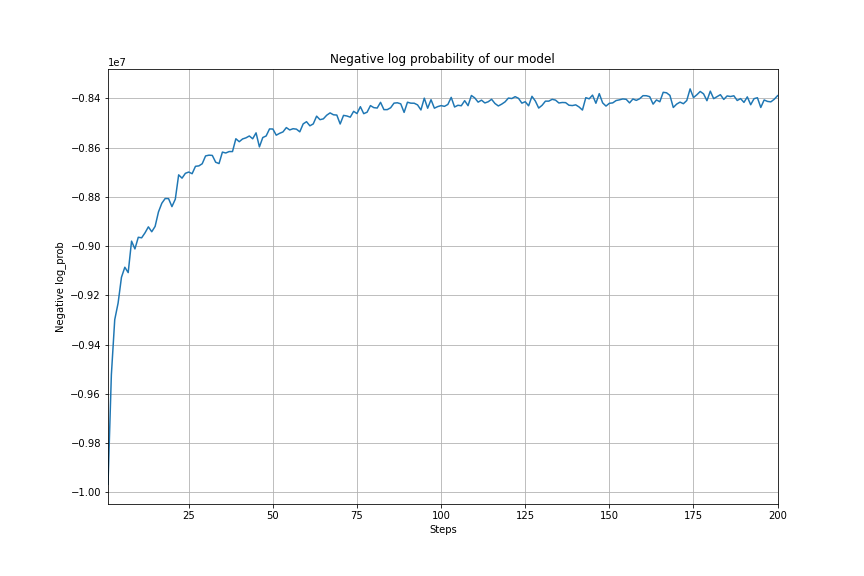
\includegraphics[width=0.50\textwidth]{figures/0908/log_prob_20t}}%
\hfill
\subcaptionbox{Negative ELBO}{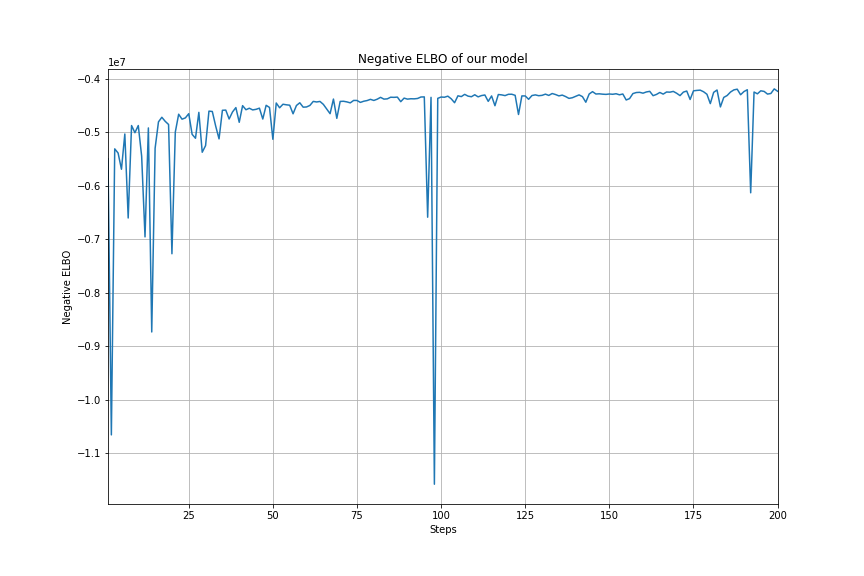
\includegraphics[width=0.50\textwidth]{figures/0908/elbo_20t}}%
\hfill
\caption{20Newsgroups (k=20)}
\label{fig:loss_20ng_20t}
\end{figure}
\begin{figure}
\centering
\subcaptionbox{Log probability}{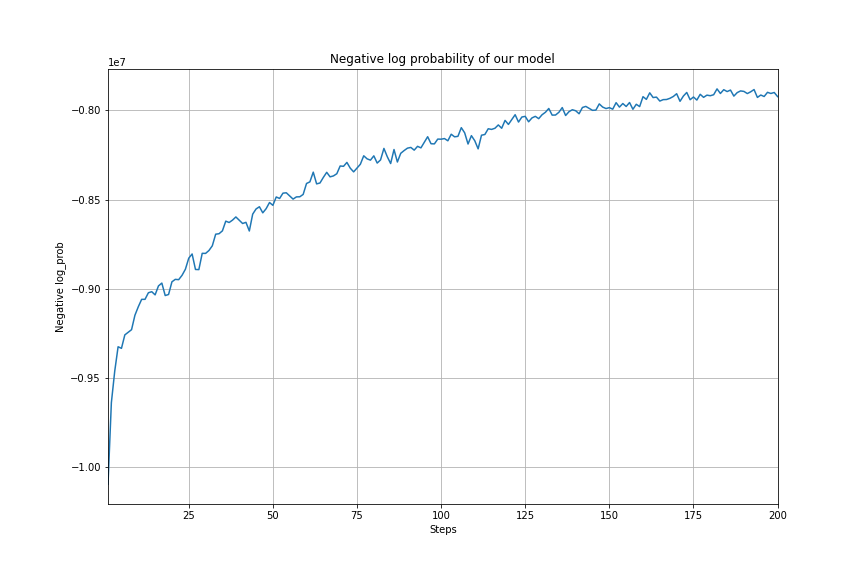
\includegraphics[width=0.50\textwidth]{figures/0908/log_prob_50t}}%
\hfill
\subcaptionbox{Negative ELBO}{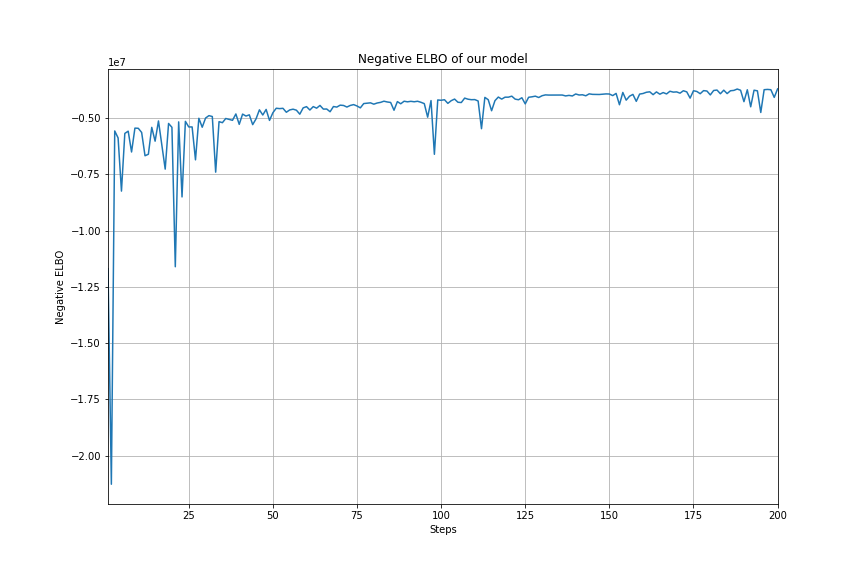
\includegraphics[width=0.50\textwidth]{figures/0908/elbo_50t}}%
\hfill
\caption{20Newsgroups (k=50)}
\label{fig:loss_20ng_50t}
\end{figure}
\begin{figure}
\centering
\subcaptionbox{Topic Diversity}{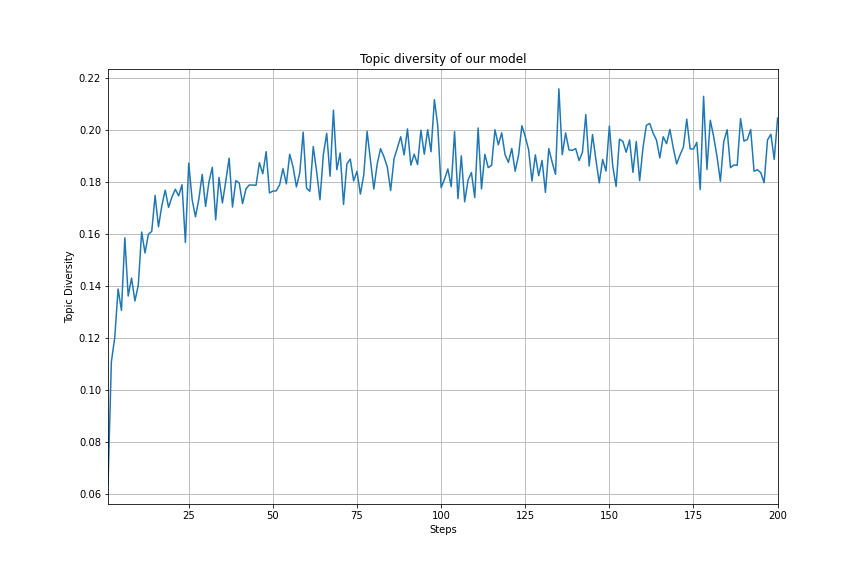
\includegraphics[width=0.50\textwidth]{figures/0908/td_20t}}%
\hfill
\subcaptionbox{Topic Coherence}{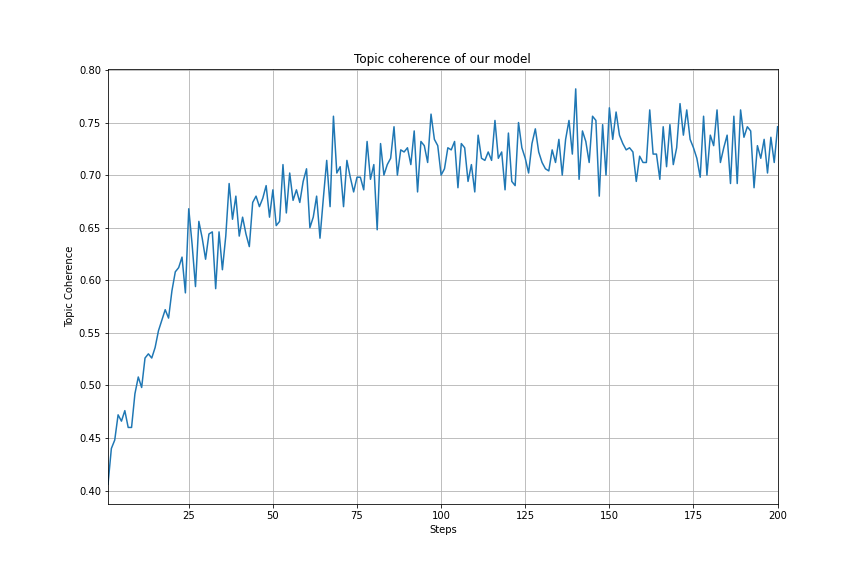
\includegraphics[width=0.50\textwidth]{figures/0908/tc_20t}}%
\hfill
\subcaptionbox{Perplexity}{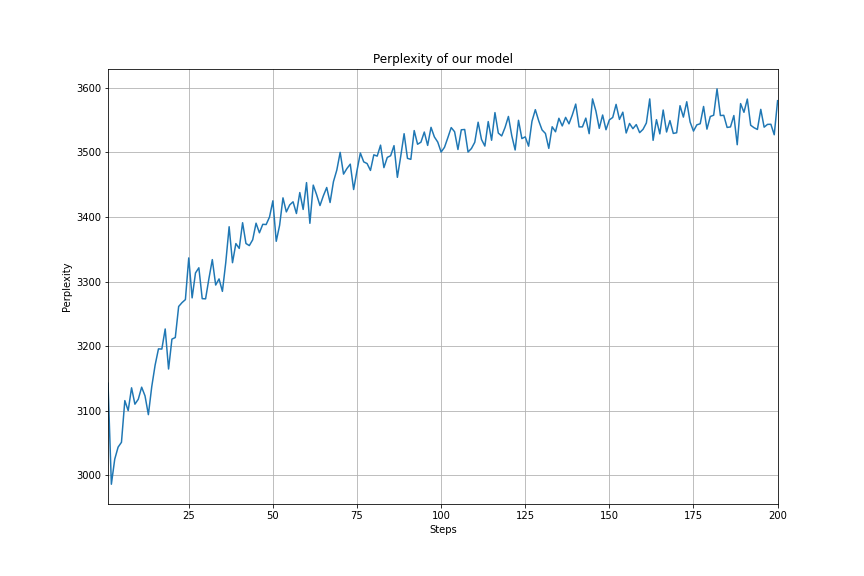
\includegraphics[width=0.50\textwidth]{figures/0908/ppl_20t}}%
\hfill
\caption{20Newsgroups (k=20)}
\label{fig:eval_20ng_20t}
\end{figure}
\begin{figure}
\centering
\subcaptionbox{Topic Diversity}{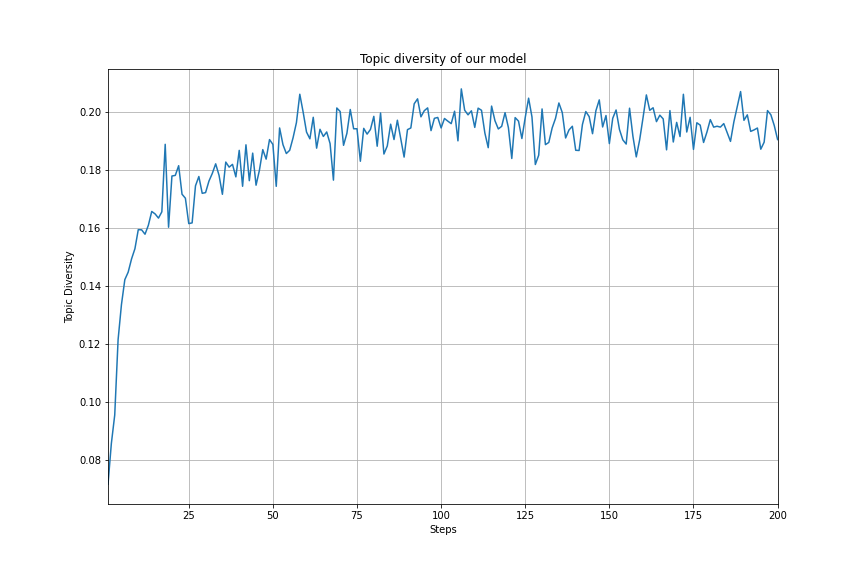
\includegraphics[width=0.50\textwidth]{figures/0908/td_50t}}%
\hfill
\subcaptionbox{Topic Coherence}{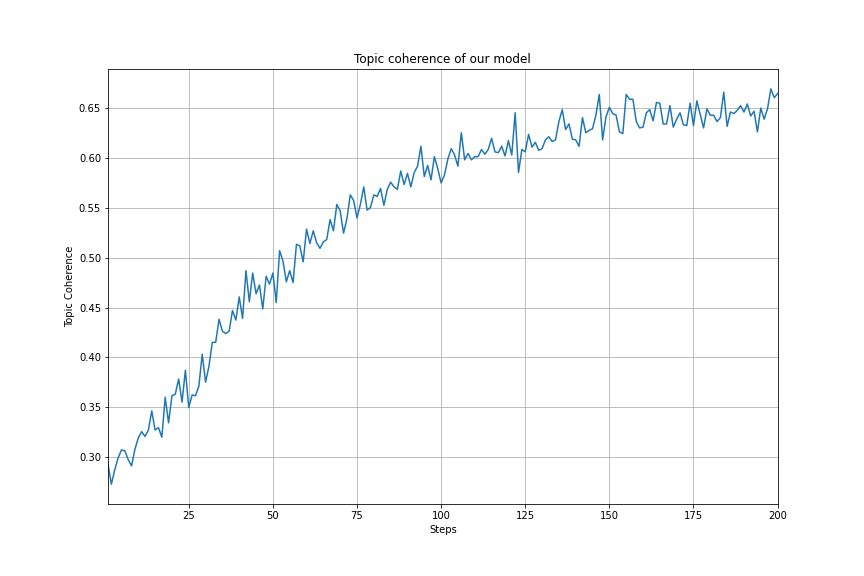
\includegraphics[width=0.50\textwidth]{figures/0908/tc_50t}}%
\hfill
\subcaptionbox{Perplexity}{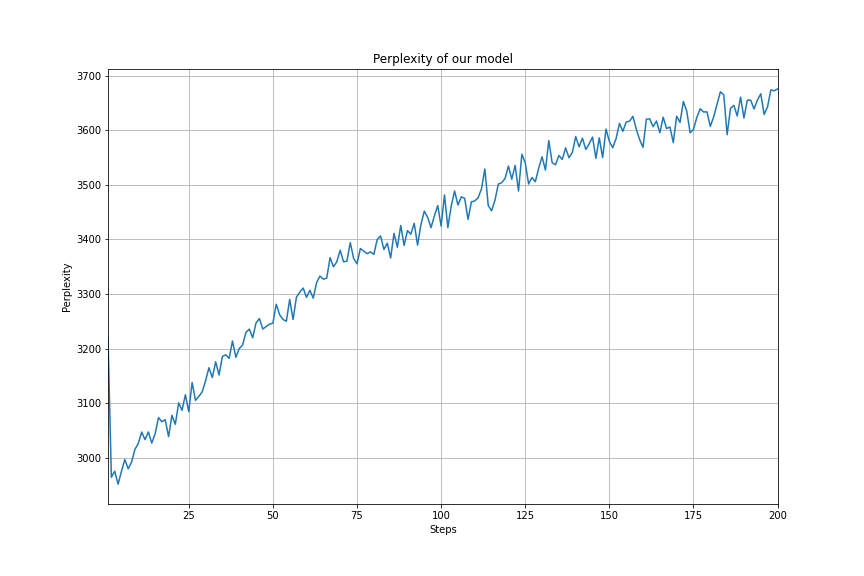
\includegraphics[width=0.50\textwidth]{figures/0908/ppl_50t}}%
\hfill
\caption{20Newsgroups (k=50)}
\label{fig:eval_20ng_50t}
\end{figure}
\subsection{Visualization}
To clearly demonstrate the representation for , we applied t-SNE to map the topic-word representation into 2-dimension continuous space. In figure \ref{fig:tsne20t25w2} and \ref{fig:tsne50t25w0}, demonstrate the t-SNE visualization of the topic-word distribution for 20Newsgroups for k=20 and k=50.
\begin{figure}
\centering
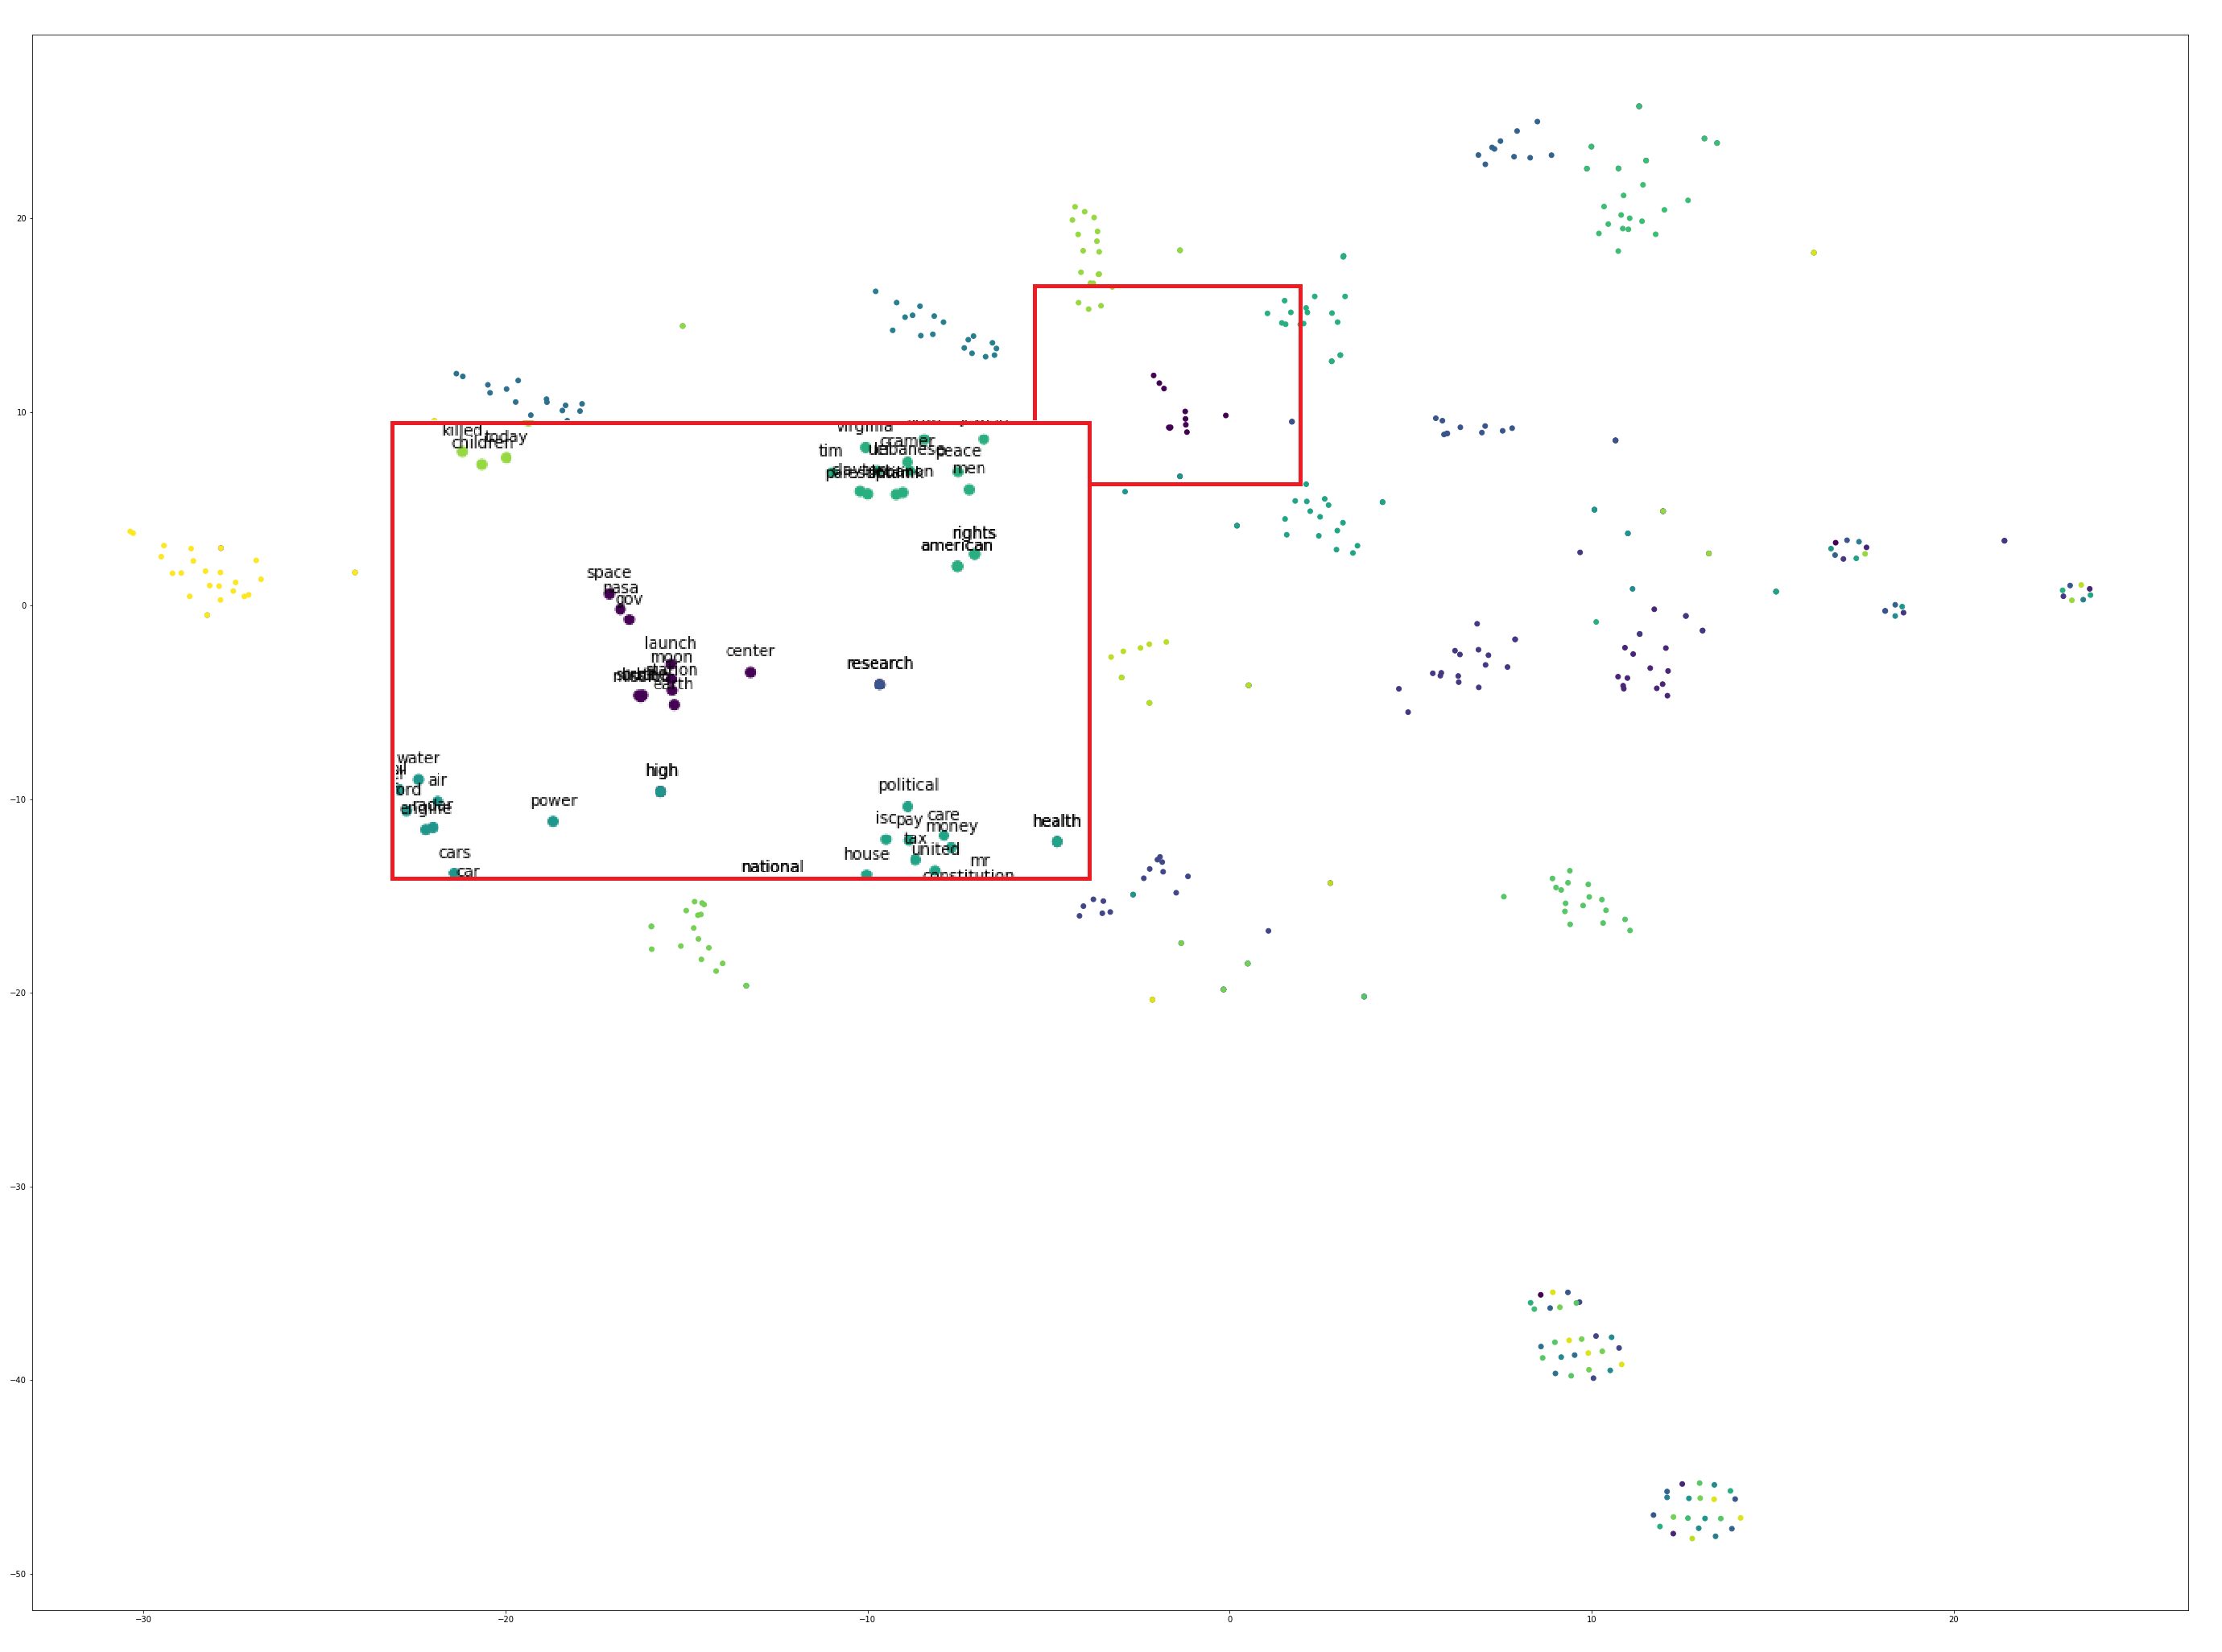
\includegraphics[width=1\linewidth]{figures/0908/tsne_20t_25w_2}
\caption{Visualization \#Topics:20}
\label{fig:tsne20t25w2}
\end{figure}
\begin{figure}
\centering
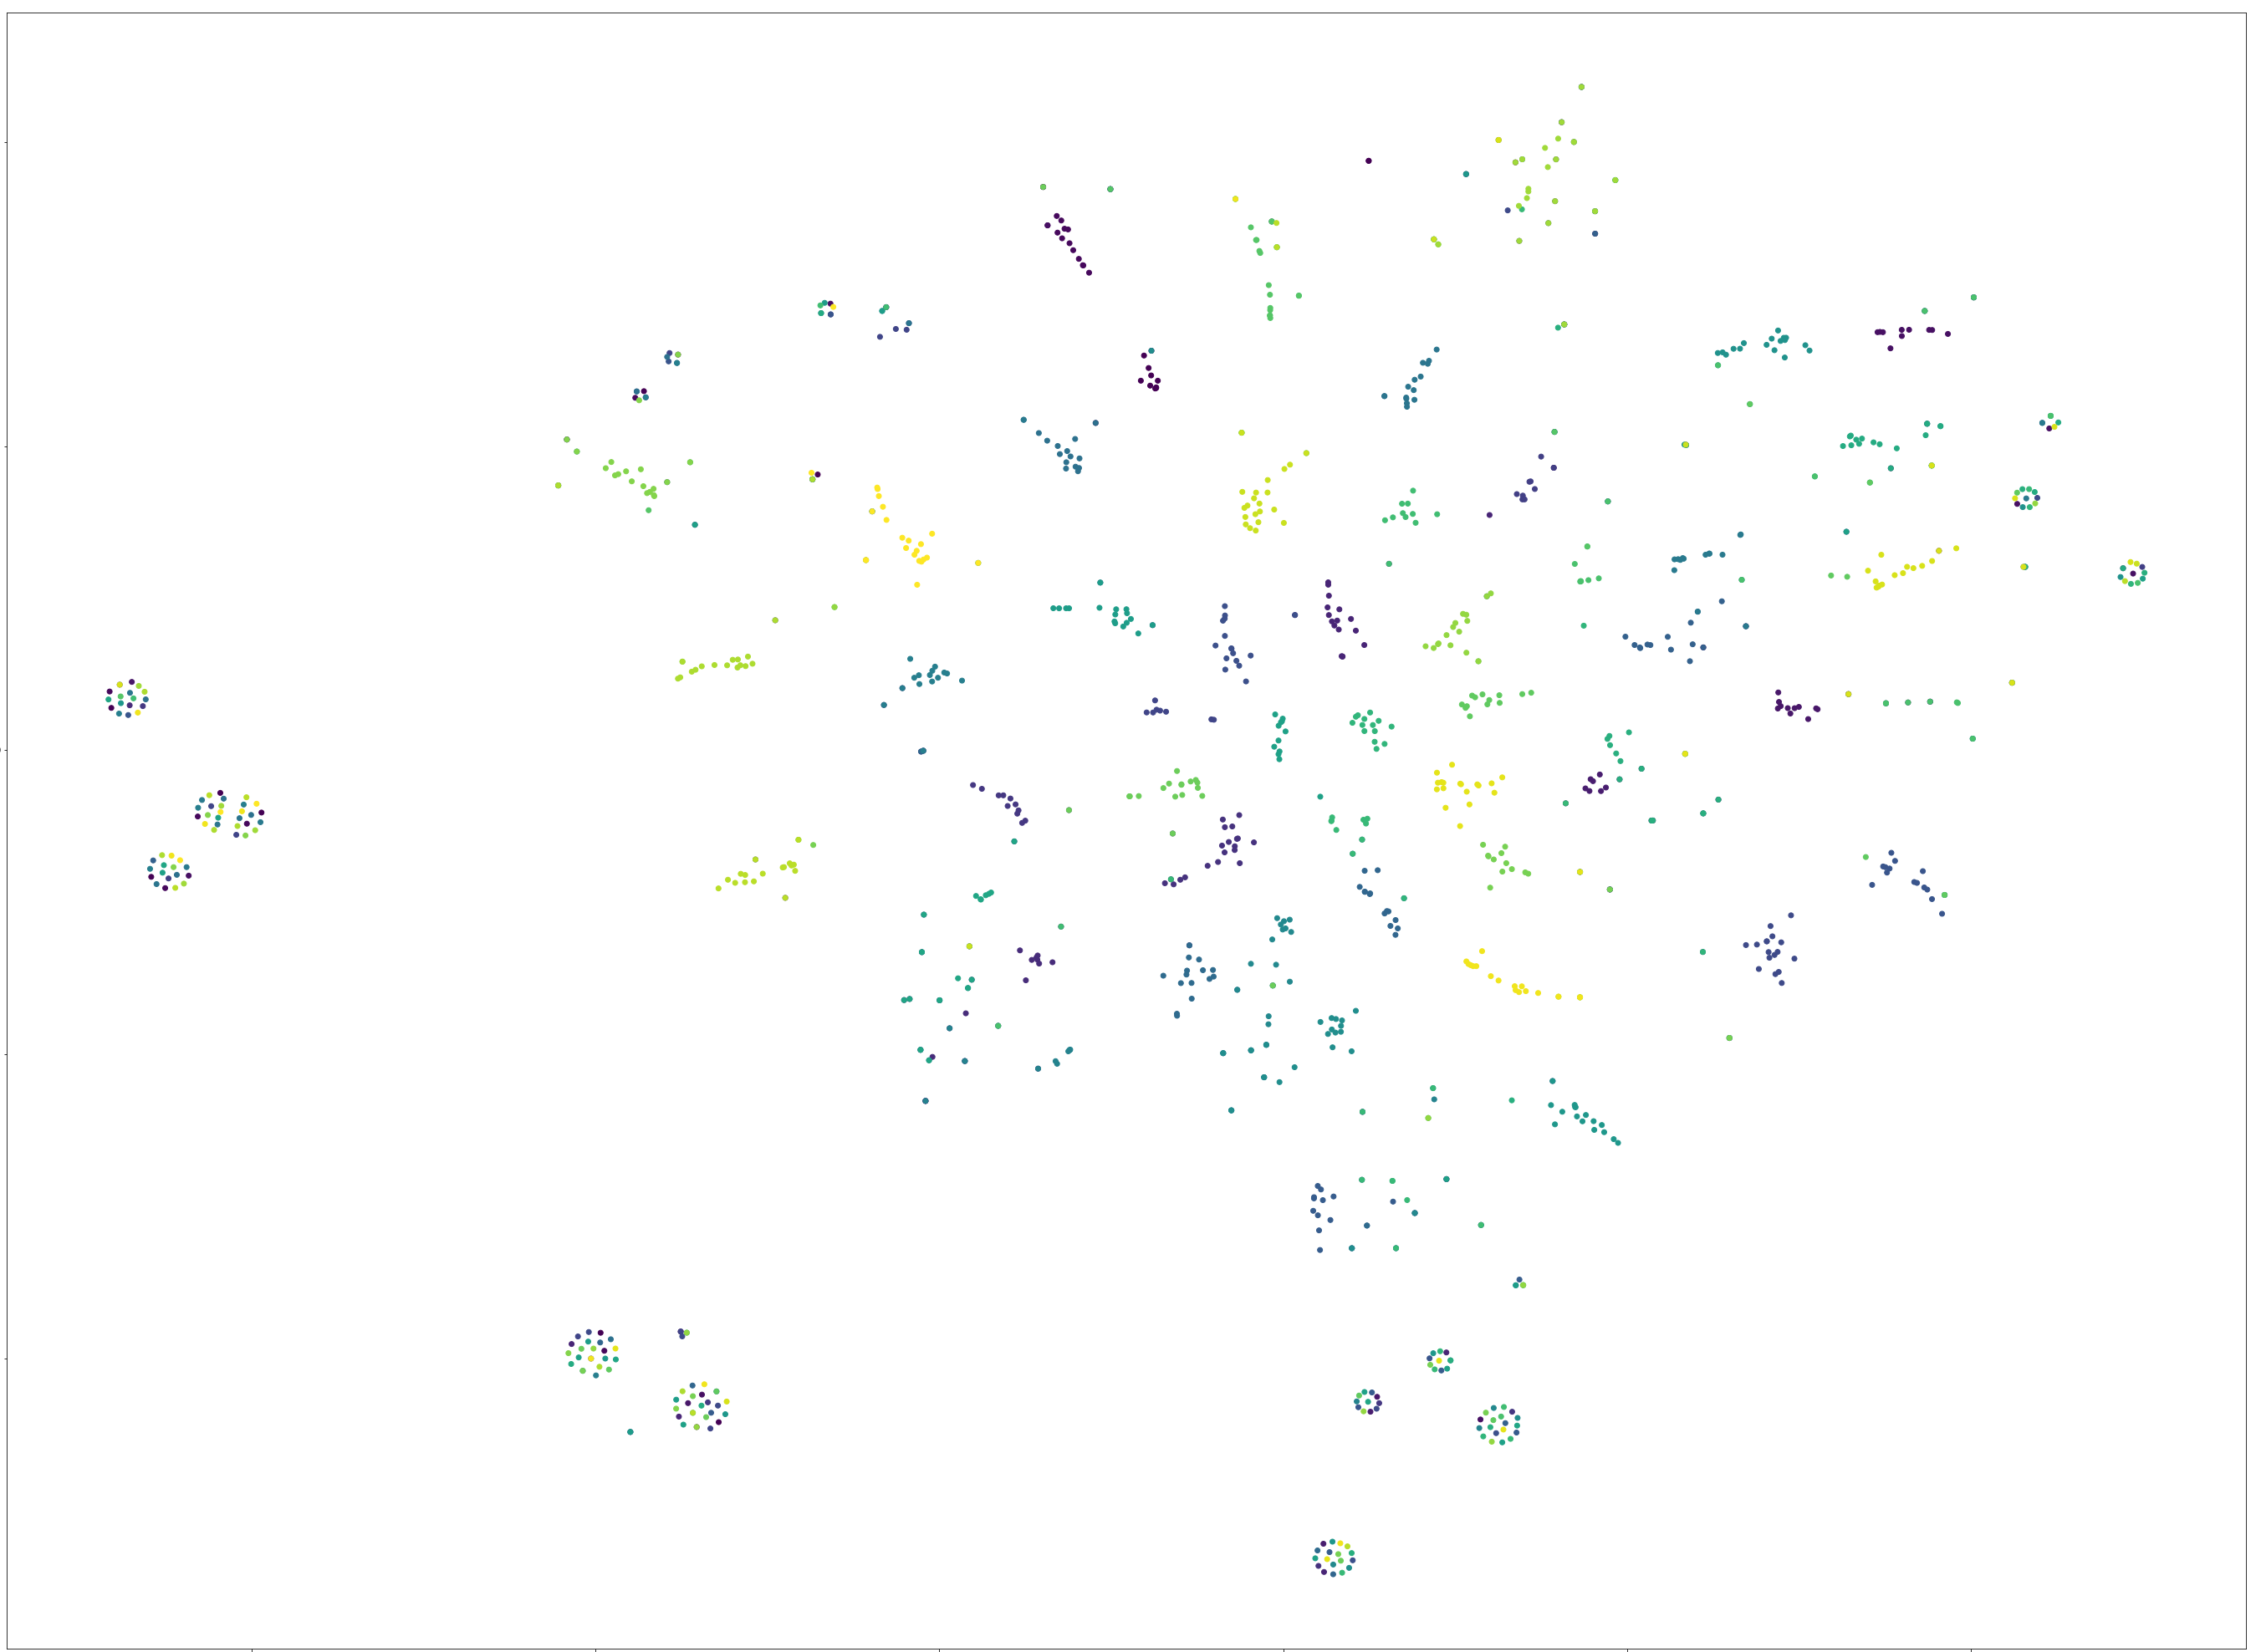
\includegraphics[width=1\linewidth]{figures/0908/tsne_50t_25w_0}
\caption{Visualization \#Topics:50}
\label{fig:tsne50t25w0}
\end{figure}
